\documentclass[11pt,a4paper]{article}
\usepackage{fontspec}
\setmainfont{DejaVu Serif}
\setsansfont{DejaVu Sans}
\setmonofont{DejaVu Sans Mono}
\usepackage{polyglossia}
\setdefaultlanguage{ukrainian}
\usepackage[a4paper,top=2.2cm,bottom=2.2cm,left=2.3cm,right=2.3cm]{geometry}
\usepackage{amsmath,amssymb,booktabs,array,graphicx,float,xcolor,hyperref,microtype}
\hypersetup{colorlinks=true,allcolors=blue}
\graphicspath{{figures/}}
\newcommand{\CI}[2]{[#1,\,#2]}
\title{\textbf{Експеримент 06: механістична декомпозиція похибки}\\[0.35em]
\large Causal ablation для двошарової CTMC апроксимації}
\author{}
\date{11 серпня 2026}
\begin{document}
\maketitle

\begin{abstract}
Мета експерименту --- з'ясувати, \emph{звідки саме} береться розбіжність між Full Micro CTMC та двошаровою Micro--Macro апроксимацією, а не просто підібрати коригувальний коефіцієнт. Ми розкладаємо похибку на втрату інформації про стан source-side boundary, стан destination-side boundary, edge-level source--target сполучення, placement імпорту, повторні імпорти та окремо враховуємо вже встановлену production-scheduler discrepancy. Основний дизайн використовує 100 paired мереж з CE-01: $L=10$, $n=100$, $d\approx6$, $k=5$, $\beta_{in}=\beta_{out}=0.003$, SI, $T_{end}=4000$.

Найсильніші результати: source-boundary state дає покращення $+105.12$ RMST відносно aggregate/uniform baseline, 95\% CI $\CI{+2.81}{+207.14}$; exact edge-conditioned placement після exact hazard дає $+168.77$, CI $\CI{+62.04}{+275.35}$. Destination marginal окремо та edge-pair covariance не мають детектованого ефекту в базовій комірці. Комбінація source+destination boundary margins із boundary-local placement відтворює Full Micro на базовій комірці з $\Delta RMST=+10.06$, CI $\CI{-83.67}{+105.12}$, а на незалежній near/random/far gateway-перевірці значно зменшує topology-induced sign flip.
\end{abstract}

\section{Питання дослідження}
Замість питання ``який correction factor зменшує bias?'' ставимо причинне питання: \emph{яку конкретну інформацію втрачає двошарова апроксимація і який внесок цієї втрати у похибку часу поширення?}

Важливе обмеження архітектури: макрорівень не повинен знати внутрішню структуру спільноти --- node identities, internal edges чи точне положення gateway-вузлів. Тому oracle arms нижче використовуються лише як діагностичні інтервенції. Якщо oracle показує, що певна інформація критична, наступний крок --- передавати її через мінімальний скалярний interface state, який обчислюється всередині micro-level.

\section{Передумова: дві різні класи похибки}
Попередній synchronization audit уже показав, що поточний production MicroMacro має окрему реалізаційну/семантичну розбіжність з event-driven реалізацією того самого aggregate hazard. На тих самих 100 paired реплікаціях:
\begin{center}
\begin{tabular}{lrr}
\toprule
Модель & RMST & $\Delta$RMST vs Full Micro\\
\midrule
Full Micro & 2936.73 & 0\\
Event-driven aggregate & 2715.94 & -220.79\\
Production $\tau=0.25$ & 1708.71 & -1228.03\\
Production $\tau=0.5$ & 1695.17 & -1241.56\\
Production $\tau=1$ & 1677.55 & -1259.18\\
\bottomrule
\end{tabular}
\end{center}
Отже, цей Experiment 06 навмисно аналізує \textbf{event-driven structural approximation error}; production scheduler треба виправляти окремо. Інакше structural correction буде компенсувати implementation error.

\section{Механістичний дизайн}
Для пари спільнот $i\to j$ позначимо сумарну вагу міжспільнотних ребер $W_{ij}$. Поточний aggregate hazard:
\begin{equation}
\lambda^{A}_{ij}=\beta W_{ij}\frac{I_i}{N_i}\frac{S_j}{N_j}.
\end{equation}
Вводимо дві boundary marginals, що обчислюються локально на micro-level:
\begin{align}
B^{I}_{ij}(t)&=\sum_{(u,v)\in E_{ij}} w_{uv}\,\mathbf 1\{u\text{ infected}\},\\
B^{S}_{ij}(t)&=\sum_{(u,v)\in E_{ij}} w_{uv}\,\mathbf 1\{v\text{ susceptible}\}.
\end{align}
Тоді абляційні hazards:
\begin{align}
\lambda^{S}_{ij}&=\beta B^{I}_{ij}\frac{S_j}{N_j},\\
\lambda^{D}_{ij}&=\beta \frac{I_i}{N_i}B^{S}_{ij},\\
\lambda^{SD}_{ij}&=\beta\frac{B^{I}_{ij}B^{S}_{ij}}{W_{ij}},\\
\lambda^{E}_{ij}&=\beta\sum_{(u,v)\in E_{ij}}w_{uv}\mathbf 1\{u\text{ infected}\}\mathbf 1\{v\text{ susceptible}\}.
\end{align}
$\lambda^{SD}\to\lambda^{E}$ ізолює edge-pair joint/covariance, тоді як $A\to S$ і $A\to D$ ізолюють source- та destination-side boundary state.

\subsection{Варіанти}
\begin{center}
\small
\begin{tabular}{lll}
\toprule
ID & Hazard information & Placement\\
\midrule
A/U & community prevalence & uniform susceptible\\
S/U & infected source-boundary weight & uniform susceptible\\
D/U & susceptible destination-boundary weight & uniform susceptible\\
SD/U & source+destination boundary marginals & uniform susceptible\\
E/U & exact active cross-edge hazard & uniform susceptible\\
E/E & exact active cross-edge hazard & exact edge-conditioned\\
S/B & source-boundary hazard & boundary-local\\
SD/B & source+destination marginals & boundary-local\\
\bottomrule
\end{tabular}
\end{center}

\section{Основна 2$\times$2 декомпозиція: результати}
\begin{figure}[H]\centering
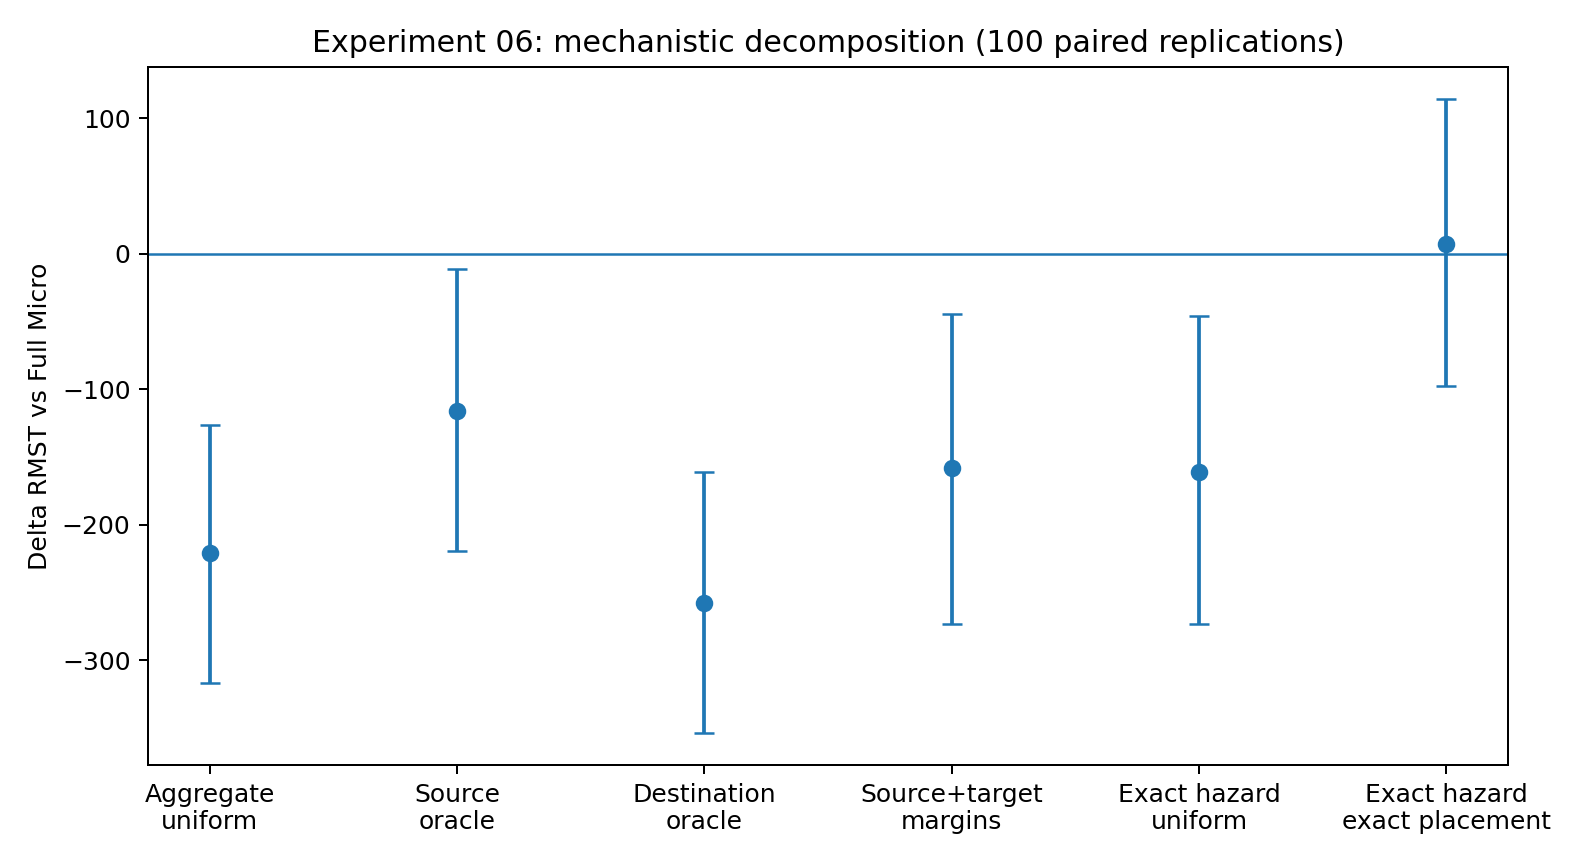
\includegraphics[width=.92\linewidth]{mechanistic_ladder.png}
\caption{Зсув RMST відносно Full Micro; 100 paired реплікацій, paired bootstrap 95\% CI.}
\end{figure}

\begin{table}[H]\centering\small
\begin{tabular}{lrrr}
\toprule
Варіант & RMST & $\Delta$RMST vs Full Micro & 95\% CI\\
\midrule
A/U & 2715.94 & -220.79 & $\CI{-316.87}{-126.37}$\\
S/U & 2821.06 & -115.68 & $\CI{-218.90}{-11.36}$\\
D/U & 2679.35 & -257.38 & $\CI{-353.81}{-160.74}$\\
SD/U & 2778.88 & -157.85 & $\CI{-273.27}{-44.54}$\\
E/U & 2775.50 & -161.23 & $\CI{-273.31}{-45.52}$\\
E/E & 2944.27 & +7.54 & $\CI{-97.52}{+114.44}$\\
Full Micro & 2936.73 & 0 & ---\\
\bottomrule
\end{tabular}
\caption{Термінальний RMST для останнього шару. Completion=1 для всіх варіантів.}
\end{table}

\subsection{Каузальні paired contrasts}
\begin{table}[H]\centering\small
\begin{tabular}{p{6.1cm}rr}
\toprule
Інтервенція & $\Delta$RMST & 95\% CI\\
\midrule
A/U $\to$ S/U: source-boundary state & +105.12 & $\CI{+2.81}{+207.14}$\\
A/U $\to$ D/U: destination-boundary state & -36.59 & $\CI{-141.59}{+65.57}$\\
A/U $\to$ SD/U: обидві marginals & +62.94 & $\CI{-38.89}{+162.74}$\\
S/U $\to$ SD/U: destination given source & -42.17 & $\CI{-106.51}{+24.44}$\\
D/U $\to$ SD/U: source given destination & +99.53 & $\CI{+15.78}{+178.55}$\\
SD/U $\to$ E/U: edge-pair joint/covariance & -3.38 & $\CI{-56.89}{+49.11}$\\
E/U $\to$ E/E: exact placement & +168.77 & $\CI{+62.04}{+275.35}$\\
Source$\times$destination interaction & -5.59 & $\CI{-130.66}{+116.80}$\\
\bottomrule
\end{tabular}
\caption{Контрасти --- різниця outcome після мінус до інтервенції. Ефекти не слід складати як незалежні частки: CTMC нелінійна і placement взаємодіє з hazard.}
\end{table}

\paragraph{Висновок 1: source-side boundary state підтримується даними.}
Коли aggregate prevalence замінюємо реальною зараженістю source-side boundary, propagation стає пізнішою на 105.1 одиниці RMST, і CI ледве, але не перетинає нуль. Це узгоджується з механізмом premature leakage: $I_i/N_i>0$ не означає, що інфекція вже досягла експортного інтерфейсу.

\paragraph{Висновок 2: destination marginal сама по собі не виправляє bias.}
D/U навіть має більш ранню point estimate, але CI для контрасту A/U$\to$D/U охоплює нуль. Це не доводить, що destination state ніколи не потрібен; у базовій SI-комірці susceptible destination boundary переважно доступний, тому source timing є жорсткішим bottleneck.

\paragraph{Висновок 3: edge-pair covariance не є головним залишком у цій комірці.}
SD/U та E/U майже однакові: контраст -3.38 із широким CI навколо нуля. Тобто після знання двох boundary margins точне спарювання ``який infected source з'єднаний з яким susceptible target'' майже нічого не додає для terminal RMST тут.

\paragraph{Висновок 4: placement --- великий механізм, але лише в правильному контексті.}
При exact hazard заміна uniform placement на exact edge-conditioned дає +168.77 RMST. Це підтверджує CE-01: placement error маскується, коли hazard вже сильно неправильний.

\section{Чи потрібен exact placement? Boundary-local ablation}
Оскільки exact placement потребує edge identities, перевірено слабший варіант: macro не вибирає вузол; destination micro-level сам локально обирає susceptible boundary node. Макро бачить лише aggregate interface state.

\begin{figure}[H]\centering
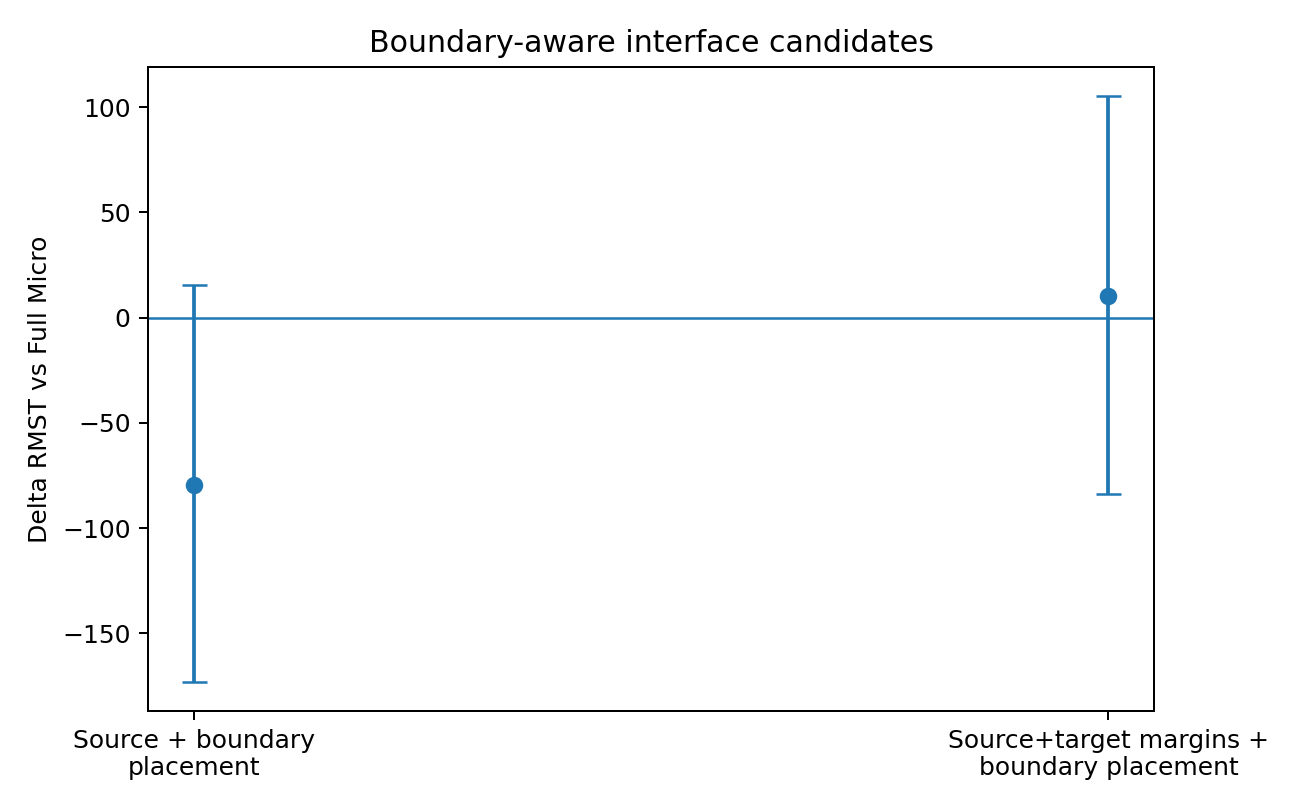
\includegraphics[width=.82\linewidth]{boundary_candidates.png}
\caption{Boundary-aware interface candidates відносно Full Micro.}
\end{figure}

Для S/B маємо $\Delta RMST=-79.55$, CI $\CI{-173.12}{+15.41}$. Для SD/B --- $+10.06$, CI $\CI{-83.67}{+105.12}$. Перехід SD/U$\to$SD/B дає +167.91, CI $\CI{+57.14}{+276.94}$. Отже, в базовій комірці \textbf{boundary-local placement достатній, щоб наблизити oracle E/E без передачі exact edge identity макрорівню}.

Це важливіше за простий correction factor: результат підказує інтерфейс між рівнями, а не калібрування конкретної мережі.

\section{Repeated-import ablation}
Щоб перевірити гіпотезу, що помилка накопичується через повторні імпорти у вже заражену спільноту, запущено single-entry варіанти: після першого зараження target community усі наступні macro imports у неї забороняються.

Нормальний A/U$-$E/U hazard gap дорівнює -59.56, CI $\CI{-158.44}{+40.92}$. У single-entry режимі gap -79.07, CI $\CI{-199.14}{+38.86}$. Зміна gap після видалення re-imports = -19.51, CI $\CI{-151.20}{+105.00}$. Отже, \textbf{немає статистичної підтримки, що repeated imports є основним джерелом baseline hazard discrepancy}.

\section{Out-of-sample gateway validation}
Найважливіша перевірка --- чи boundary interface працює не лише на одній випадковій архітектурі. Використано незалежний дизайн $L=5$, $n=100$, $d\approx6$, $k=5$, 100 paired replications для кожного режиму gateway separation: near, random, far. Макро-visible $W,n,d,k$ залишаються тими самими; прихована gateway architecture змінюється.

\begin{figure}[H]\centering
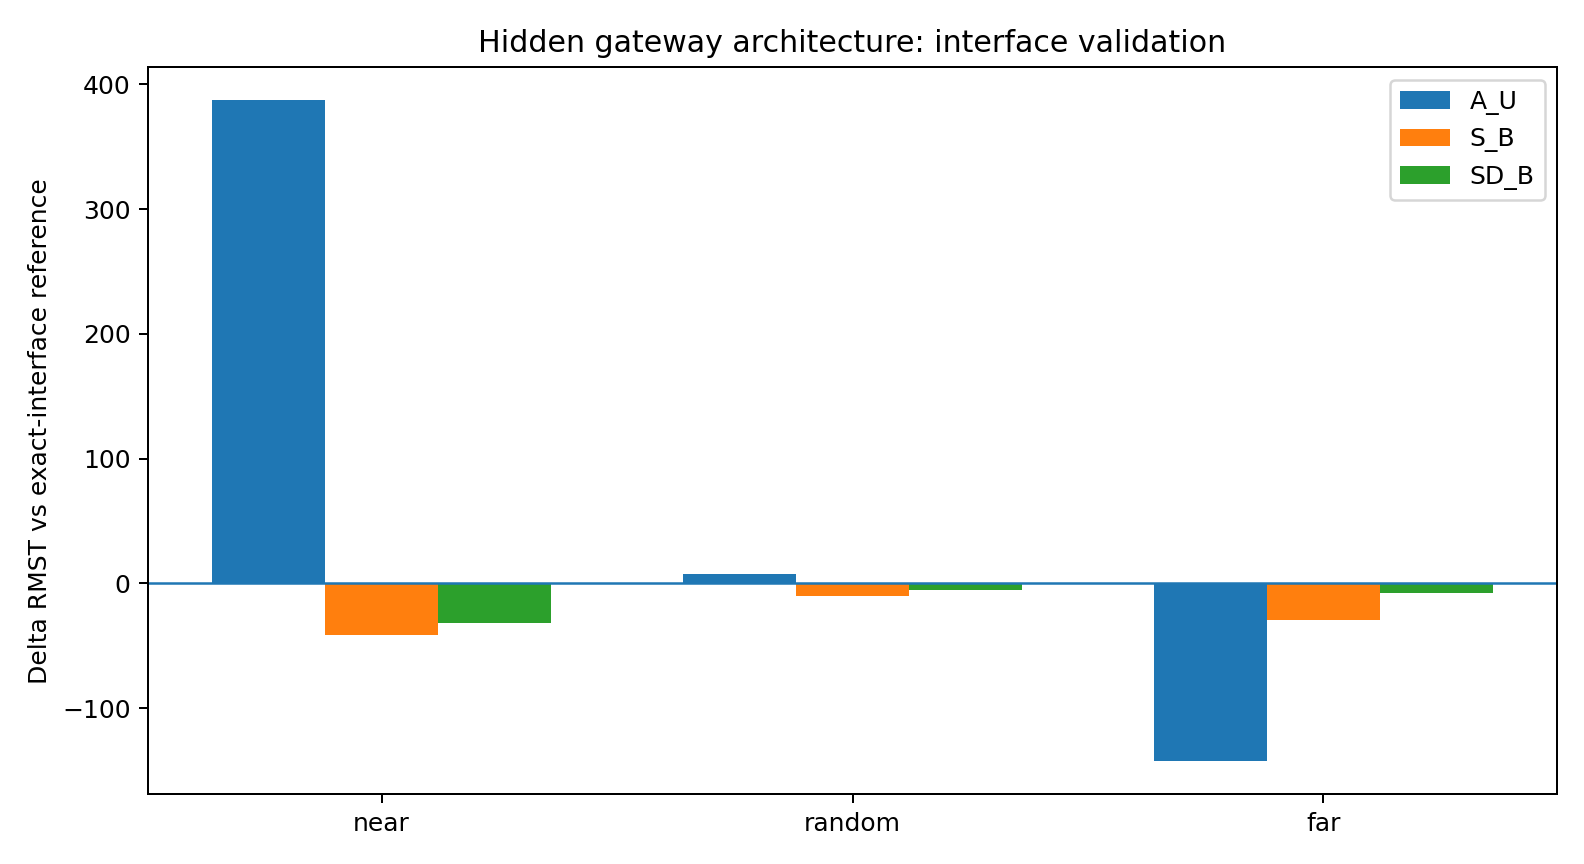
\includegraphics[width=.92\linewidth]{gateway_validation.png}
\caption{Похибка відносно event-driven exact-interface reference (E/E) у трьох прихованих gateway-архітектурах.}
\end{figure}

\begin{table}[H]\centering\small
\begin{tabular}{llrrr}
\toprule
Gateway & Model & RMST & $\Delta$ vs E/E & 95\% CI\\
\midrule
near & A/U & 1269.07 & +387.19 & $\CI{+336.93}{+434.80}$\\
near & S/B & 840.58 & -41.29 & $\CI{-77.00}{-5.41}$\\
near & SD/B & 849.89 & -31.98 & $\CI{-67.68}{+2.27}$\\
\addlinespace
random & A/U & 1269.07 & +7.65 & $\CI{-59.31}{+80.11}$\\
random & S/B & 1251.28 & -10.14 & $\CI{-66.77}{+47.45}$\\
random & SD/B & 1256.16 & -5.25 & $\CI{-53.22}{+41.40}$\\
\addlinespace
far & A/U & 1269.07 & -142.60 & $\CI{-208.57}{-78.15}$\\
far & S/B & 1382.30 & -29.37 & $\CI{-71.21}{+15.04}$\\
far & SD/B & 1404.22 & -7.44 & $\CI{-54.01}{+37.78}$\\
\bottomrule
\end{tabular}
\caption{Event-driven E/E reference RMST: near 881.87, random 1261.42, far 1411.67.}
\end{table}

Aggregate A/U дає \emph{один і той самий} RMST 1269.07 у всіх трьох режимах, бо прихована gateway architecture не входить у його observable state. Exact-interface reference змінюється майже на 530 одиниць між near і far. Через це знак aggregate bias змінюється: дуже пізній у near, майже нульовий у random, передчасний у far.

SD/B відтворює цю залежність: point errors -31.98, -5.25, -7.44. Для near і far це закриває приблизно 91.7\% та 94.8\% абсолютного A/U gap; у random baseline gap і так майже нульовий, тому ``percent closure'' нестабільний і неінформативний.

\section{Що це означає для розділення рівнів}
Результат \textbf{не означає}, що macro layer має отримати micro graph. Навпаки, дані підтримують такий interface contract:
\begin{enumerate}
\item Source micro-level локально обчислює скаляр $B^I_{ij}(t)$ --- скільки cross-boundary capacity зараз заражено.
\item Destination micro-level локально обчислює $B^S_{ij}(t)$ --- скільки boundary capacity зараз susceptible.
\item Macro-level використовує лише $W_{ij}$ та ці агреговані скаляри, наприклад $\lambda_{ij}=\beta B^I_{ij}B^S_{ij}/W_{ij}$.
\item Коли macro event приходить у community $j$, сам micro-level $j$ робить boundary-local placement; node identity не виходить за межі micro-level.
\end{enumerate}
Таким чином, структуру не передаємо, але передаємо \emph{динамічний стан інтерфейсу}. Gateway experiment показує, чому без будь-якого такого сигналу універсальна точність принципово недосяжна: однакові macro observables відповідають різним microscopic outcomes.

\section{Ієрархія джерел похибки після Experiment 06}
\begin{enumerate}
\item \textbf{Production scheduler / synchronization semantics --- найбільша практична розбіжність у поточному коді.} Її треба виправити першою; зменшення $\tau$ від 1 до 0.25 саме по собі проблему не прибирає.
\item \textbf{Hidden source-interface state --- причинно підтриманий structural mechanism.} Aggregate prevalence не знає, чи інфекція досягла export boundary.
\item \textbf{Placement / import localization --- причинно підтриманий і великий, але context-dependent mechanism.} Boundary-local placement є перспективною topology-private заміною exact edge placement.
\item \textbf{Destination boundary susceptibility --- не підтримана як окремий великий effect у baseline SI}, але корисна у симетричному SD interface і може стати важливішою при SIR/depletion.
\item \textbf{Edge-pair covariance --- не детектована як важливий terminal-RMST effect у baseline cell.}
\item \textbf{Repeated imports --- не підтримані як головна причина baseline hazard gap.}
\end{enumerate}

\section{Обмеження}
\begin{itemize}
\item Основна decomposition cell --- SI, sparse random-connected chain. Не можна переносити нульові ефекти destination/covariance на всі режими.
\item SIR з recovery/extinction треба перевірити окремо; там destination susceptibility та repeated import можуть стати важливішими.
\item Oracle arms мають доступ до hidden micro state всередині експериментального simulator. Їх призначення --- причинна діагностика, не готовий production API.
\item Gateway validation використовує E/E як event-driven exact-interface reference; це не новий direct Full-Micro run у цій supplemental гілці.
\item Paired bootstrap CIs стосуються outcome contrasts у конкретному дизайні; ``gap closure'' є descriptive point estimate, не окремою causal fraction.
\end{itemize}

\section{Рекомендований наступний експеримент}
Не розробляти ще один глобальний correction coefficient. Наступний крок --- \textbf{Experiment 07: interface-contract validation}:
\begin{enumerate}
\item реалізувати production-safe API, де micro layer повертає лише $B^I$/$B^S$ scalars, а placement залишається локальним;
\item спочатку вирівняти production scheduler semantics з event-driven reference;
\item після цього перевірити SD/B interface на $r=\beta_{out}/\beta_{in}\in\{0.5,1,2\}$, $d$, $k$, кількох topology families;
\item окремо SIR: RMST, completion/extinction probability, rel-$W_1$, layerwise arrivals;
\item використовувати held-out topology validation, а не in-sample calibration.
\end{enumerate}

\section{Фінальний висновок}
Experiment 06 дає механістичну відповідь, а не просто емпіричну кореляцію. У базовому event-driven режимі головна втрата інформації в hazard --- \textbf{чи інфекція реально дійшла до source boundary}; після достатньо правильного hazard великим другим механізмом стає \textbf{де саме всередині destination community відбувається import}. Точна edge-level структура для цього не обов'язково має виходити на macro level: source/destination boundary marginals плюс boundary-local placement відтворюють baseline Full Micro і значно краще поводяться на прихованих near/random/far gateway architectures.

Це одночасно пояснює попередню нестабільність корекцій: вони намагалися відновити динамічний hidden interface state зі статичних або загальних aggregate descriptors. Правильний напрям --- не ``вгадувати'' структуру на macro level, а визначити мінімальний динамічний контракт між двома чорними скриньками.

\section*{Відтворення}
Основний runner: \texttt{extrascripts/run\_mechanistic\_error\_decomposition.py}.\\
Supplements: \texttt{run\_reimport\_ablation.py}, \texttt{run\_boundary\_placement\_context.py}, \texttt{run\_gateway\_interface\_validation.py}.\\
Нові outputs: \texttt{output/mechanistic\_error\_decomposition/}.\\
Архівні paired baselines: \texttt{output/ablation\_hazard\_placement/final\_100/}.

\end{document}
